\chapter{Análisis léxico}
\section{¿Cuando interesa utilizar un Procesador de Lenguajes?}
Cuando quiero hacer la comunicación en un sistema y dicha comunicación es compleja, hay ocasiones donde me interesa definir un lenguaje con un dominio físico.

\section{¿Cuál es la función del analizador léxico?}
Es función del analizador léxico: 
\begin{itemize}
	\item Reconocer los símbolos o tokens que componen el texto fuente.
	\item Eliminar comentarios del texto fuente.
	\item Eliminar los espacios en blanco, saltos de línea y página, tabuladores
	\item Avisar de los errores léxicos detectados.
\end{itemize}

\begin{figure}[h]
	\centering
	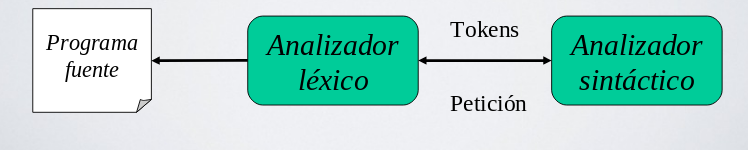
\includegraphics[width=0.7\linewidth]{img/lex1}
	\caption{}
	\label{fig:lex1}
\end{figure}

El analizador léxico es el único que interactúa con la entrada, no se detiene al encontrar los primeros errores.
\clearpage
Un ejemplo de funcionamiento del analizador léxico.
\begin{figure}[h]
	\centering
	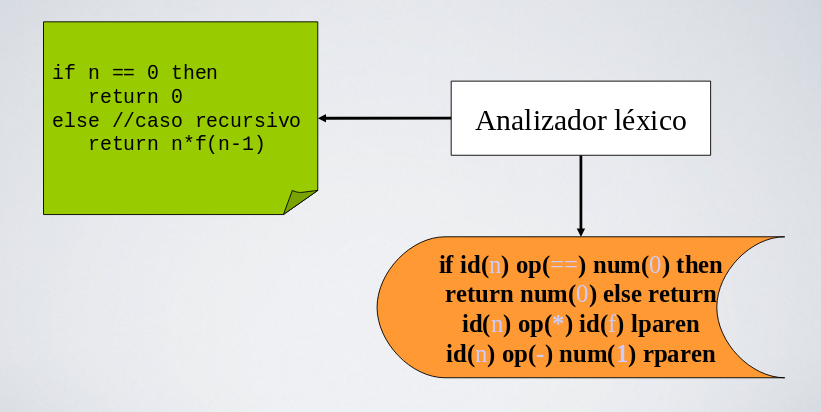
\includegraphics[width=0.7\linewidth]{img/lex2}
	\caption{}
	\label{fig:lex2}
\end{figure}

\section{Función del analizador léxico}
\begin{itemize}
	\item \textbf{Token}: un token es uno o varios elementos básicos del lenguaje fuente que tienen un significado propio. Ejemplos de tokens, presentes en todos los lenguajes de programación, identificadores, palabras reservadas,...
	\item \textbf{Lexema}: es \textit{if} por ejemplo, una combinación concreta de símbolos que forman un token.
	\item \textbf{Patrón}: regla asociada al token que describe a un conjunto de lexemas
\end{itemize}
Son símbolos terminales de la GLC que se van a encargar de comprobar que la estructura del lenguaje es válida, al analizador léxico no le importan los espacios, ni los tabuladores, solo le interesa que la secuencia sea correcta.
\newline
\newline
Es útil estudiar análisis léxico para el reconocimiento de patrones.
\newline
\newline
El problema es encontrar lexemas y disparar patrones, mediante una gramática regular especificamos los lexemas.

	\begin{center}
	\begin{tabular}{|c|c|c|}
		\hline 
		\textbf{Token} & \textbf{Lexema} & \textbf{Patrón} \\ 
		\hline 
		moore & moore & m$\cdot$o$\cdot$o$\cdot$r$\cdot$e  \\ 
		\hline 
		estados &estados & e$\cdot$s$\cdot$t$\cdot$a$\cdot$d$\cdot$o$\cdot$s \\ 
		\hline 
		estado$\_$in & estado$\_$in & e$\cdot$s$\cdot$t$\cdot$a$\cdot$d$\cdot$o$\cdot$$\_$$\cdot$i$\cdot$n \\ 
		\hline 
		alf$\_$in	& alf$\_$in & a$\cdot$l$\cdot$f$\cdot$$\_$i$\cdot$n \\ 
		\hline 
		alf$\_$out	& alf$\_$out & a$\cdot$l$\cdot$f$\cdot$$\_$o$\cdot$u$\cdot$t \\ 
		\hline 
		transicion	& transicion & t$\cdot$r$\cdot$a$\cdot$n$\cdot$s$\cdot$i$\cdot$c$\cdot$i$\cdot$o$\cdot$n \\ 
		\hline 
		comportamiento	& comportamiento & c$\cdot$o$\cdot$m$\cdot$p$\cdot$o$\cdot$r$\cdot$t$\cdot$a$\cdot$m$\cdot$i$\cdot$e$\cdot$n$\cdot$t$\cdot$o \\ 
		\hline 
		Paréntesis abierto	& ( & ( \\ 
		\hline 
		Paréntesis cerrado	& ) & ) \\ 
		\hline 
		Llave abierta	& $\{$ & $\{$ \\ 
		\hline 
		Llave cerrada	& $\}$ & $\}$ \\ 
		\hline 
		Punto y coma	& ; & ; \\ 
		\hline 
		Coma	& , &  , \\ 
		\hline
		Asterisco barra & $\ast/$  & $\ast$$\cdot/$ \\ 
		\hline 
		Barra asterisco & $/\ast$  &  $/$$\cdot$$\ast$ \\ 
		\hline  
		ID	& hola  & [A-Za-z][A-Zaz0-9$\_$]* \\ 
		\hline 
		CMP	& c1 & c[1-9][0-9]* \\ 
		\hline
		CODIGO	& $\#$codigo aquí $\#$  & $\#$$\cdot$ codigo aquí $\cdot$$\#$\\ 
		\hline
		
		
		
	\end{tabular} 	
\end{center}

\section{Ejemplos con JFlex}

TO-DO

\section{Tratamiento de errores}

TO-DO






